\documentclass{article}
\usepackage[utf8]{inputenc}

\title{Linear Algebra}
\author{Josh Joseph}
\date{Summer 2020}

\addtolength{\oddsidemargin}{-.875in}
\addtolength{\evensidemargin}{-.875in}
\addtolength{\textwidth}{1.75in}
\addtolength{\topmargin}{-.875in}
\addtolength{\textheight}{1.75in}

\usepackage{amsmath}
\usepackage{amssymb}
\usepackage{gensymb}
\usepackage{graphicx}
\usepackage{float}
\usepackage{amsthm}
\usepackage{amsbsy}
\usepackage{etoolbox}
\usepackage{esvect}

\AtBeginEnvironment{gather}{\setcounter{equation}{0}}

\renewcommand{\qedsymbol}{$\blacksquare$}
\let\oldvec\vv
\renewcommand{\vv}[1]{\oldvec{\mathbf{#1}}}
\let\oldhat\hat
\renewcommand{\hat}[1]{\oldhat{\mathbf{#1}}}
\let\vl\langle
\let\vr\rangle
\let\ve\hat
\renewcommand{\ve}[1]{\vl#1\vr}
\let\d\hat
\renewcommand{\d}{\hspace{3pt}\textrm{d}}

\makeatletter
\newcommand*\vdot{\mathpalette\vdot@{.5}}
\newcommand*\vdot@[2]{\mathbin{\vcenter{\hbox{\scalebox{#2}{$\m@th#1\bullet$}}}}}
\makeatother

\begin{document}

\maketitle

\tableofcontents
\newpage
\section{Vectors}
\subsection{The Geometry and Algebra of Vectors}
A \textbf{vector} $\vv{AB}$ is a line segment with a direction starting from \textbf{initial point} $A$ to \textbf{terminal point} $B$. For every point $B$ there is a vector $\vv{OB}$ that corresponds to the displacement from $O$ to $B$, where $O$ is the origin. \textit{Refer to MC notes for more on vectors, this is mainly a recap and summarization}.
\subsubsection{Vector Representations}
There are two main ways to represent vectors, the first is a simple \textbf{row vector} while the second is a \textbf{column vector}:
\begin{gather*}
    \vv{v} = \ve{v_x,v_y,v_z...v_n}\\
    \vv{v} = \begin{bmatrix}
    v_x\\
    v_y\\
    v_z\\
    \vdots\\
    v_n
    \end{bmatrix}
\end{gather*}
Two vectors are \textbf{equal} if they have the same components, or if they have the same length(magnitude) and direction. Vectors normally start in the \textbf{standard position}, with the tail at the origin. However, even if a vector is \textit{translated} away, equality does not depend on position.

Vector addition and subtraction are covered in MC notes.
\subsubsection{Linear Combinations}
A vector $\vv{v}$ is a \textbf{linear combination} of vectors $\vv{v_1}, \vv{v_2},\vv{v_3}...\vv{v_k}$ if there are scalars $c_1,c_2,c_3...c_k$ which \textit{combine} to form $\vv{v} = c_1\vv{v_1} + v_2\vv{v_2} + c_3\vv{v_3}...c_k\vv{v_k}$. The scalars are called the \textbf{coefficients} of linear combinations.

If $\vv{v}$ is a linear combination of vectors $\vv{v_1} \textrm{ and } \vv{v_2}$, then the coordinates of $\vv{v}$ with respect to $\vv{v_1},\vv{v_2}$ are $c_1$ and $c_2$.
\subsubsection{Binary Vectors and Modular Arithmetic}
Computers use \textit{binary} to communicate, a language made up of only $0$ and $1$. \textbf{Binary Vectors} are vectors that only have components $0$ or $1$. Using this, the rules of normal math operations must be changed so that whenever a number gets above $1$ it has to be reset down. For example, $3 \implies 1$, and $6 \implies 0$. Basically, any odd number is $1$ and even number is $0$. This binary space is denoted by $\mathbb{Z}_2$. If these vectors all have $n$ components then the space consisting of all of them is $\mathbb{Z}_2^n$, where $n$ is called the \textit{length} of the vector. Be careful not to confuse length in $\mathbb{R}$ with length in $\mathbb{Z}$.

In a similar way, the vectors in $\mathbb{Z}_3$ reset every $3$. So to find a mathematical sum of vectors in this space, add up their components and divide by $3$ and their remainder is the correct value to use. This idea is similar to a clock or a periodic function that repeats.
\subsection{Length and Angle: The Dot Product}
Note: MC notes section 13.3 goes into much more depth for the Dot Product.
\subsubsection{The Dot Product}
If $\vv{u} = \ve{u_1,u_2...u_n}$ and $\vv{v} = \ve{v_1,v_2...v_n}$, then the \textit{scalar }\textbf{dot product} of the two vectors is:
\begin{gather*}
    \vv{u} \vdot \vv{v} = u_1v_1 + u_2v_2 + ...u_nv_n
\end{gather*}
There are many important properties of the dot product, which are easily proved by expanding out the components and manipulating them. These are seen in 13.3 of MC notes. One example is $\vv{v} \vdot \vv{v} \geqslant 0$, which is true since multiplying any component(any number) by itself never yields a negative.
\subsubsection{Vector Length}
In $\mathbb{R}_2$, the distance between the origin and the point $(a,b)$ is the same as the length of the vector $\vv{v} = \ve{a,b}$, which is given by the Pythagorean Theorem, $|\vv{v}| = \sqrt{a^2 + b^2}$. Also note that $a^2 + b^2$ is the same thing as $\vv{v} \vdot \vv{v}$. So $|\vv{v}| = \sqrt{\vv{v} \vdot \vv{v}}$, which is always defined since $\vv{v} \vdot \vv{v} \geqslant 0$. This also implies that $\vv{v} \vdot \vv{v} = |\vv{v}|^2$.
\subsubsection{Unit Vectors}
Any vector with magnitude $1$ is called a unit vector. In fact, the set of all unit vectors in $\mathbb{R}_2$ is a unit circle(all points a distance $1$ from the origin. In $\mathbb{R}_3$ it is a unit sphere. Given any nonzero vector $\vv{v}$, the \textbf{unit vector} $\hat{v}$ in the $v$ direction is just the vector:
\begin{gather*}
    \hat{v} = \bigg[\dfrac{1}{|\vv{v}|}\bigg]\vv{v} = \dfrac{\vv{v}}{|\vv{v}|}
\end{gather*}
A special set of unit vectors is called the \textbf{standard unit vectors}. This set consist of all the unit vectors in $\mathbb{R}^n$ where each unit vector $\hat{e}_i$ has $i^{th}$ component $1$ and all other components $0$. In other words, all the unit vectors along the "axes" are standard unit vectors. Examples include $\hat{i},\hat{j},\hat{k}$ in $\mathbb{R}_3$.
\subsubsection{Distance}
On a number line, the distance between two points $a$ and $b$ is just $|a-b|$, the absolute value lets us ignore which is greater. This can be rewritten as $\sqrt{(a-b)^2}$ In two dimensions this formula is $\sqrt{(a_x-b_x)^2 + (a_y-b_y)^2}$. In general, this formula can be extended to $n$-dimensions:
\begin{gather*}
    \textrm{In } \mathbb{R}_n, d = \sqrt{(a_x-b_x)^2 + (a_y -b_y)^2 + (a_z-b_z)^2 +...(a_n-b_n)^2}
\end{gather*}
In terms of vectors, $d$ is just the length of $\vv{a} - \vv{b}$, which makes sense because taking $|\vv{a-b}|$ is just the square of the difference between each component of $\vv{a}$ and $\vv{b}$.
\subsubsection{Angles}
Refer to MC notes for notes on angles and direction cosines. Also, the Cauchy-Schwarz equality:
\begin{gather*}
    \vv{u} \vdot \vv{v} \leqslant |\vv{u}||\vv{v}|
\end{gather*}
This might seem easy to prove, using the cosine definition of the dot product, but note that that definition is proved using the Law of Cosines, which holds true for dimensions $n \leqslant 3$. This equality is not proved right now, but it does explain why the cosine definition works past three dimensions.

\subsubsection{Projections}
Projections and Components in MC chapter 13
\subsection{Lines and Planes}
\subsubsection{Lines}
The equation of a line in a plane is $ax +by = c$, which becomes $y = -\frac{a}{b}x + \frac{c}{b}$. Now to use vectors, we define a vector $\vv{n}$:
\begin{gather*}
    \vv{n} = \ve{a,b}\hspace{20pt}\vv{x} = \ve{x,y}\\
    \vv{n} \vdot \vv{x} = 0
\end{gather*}
The last statement is true because $\vv{n}$ represents a vector with slope that is the negative reciprocal of the line's slope: $-\frac{a}{b}$. Another way to do this is to use a \textit{parallel vector} $\vv{d} = \ve{1,-2}$. This allows us to rewrite the line's equation as:
\begin{gather*}
    \vv{x} = \vv{d}t
\end{gather*}
If the line does not pass through the origin, this equation can be modified by adding a position vector $\vv{p} = \ve{x_0,y_0,z_0}$ that gives the line's position.
\begin{gather*}
    \vv{x} = \vv{p} + \vv{d}t\\
    \vv{n} \vdot (\vv{x} - \vv{p}) = 0
\end{gather*}
Equating components gives the parametric equations of the line.
\subsubsection{Planes}
To generalize this to planes, we can defined a normal vector in $\mathbb{R}_3$ so that $\vv{n} = \ve{a,b,c}$. This also lets the following happen:
\begin{gather*}
    \vv{n} \vdot (\vv{x} - \vv{p}) = 0\\
    ax + by + cz = d
\end{gather*}
To understand why this works, imagine a line in $\mathbb{R}_2$. It can be defined by a vector perpendicular to it, which gives the slope of the line, and a point to show the line's position. Similarly in $\mathbb{R}_3$, a plane can be defined by a vector perpendicular to it, which gives all the vectors that are perpendicular to it. A point also gives the position here, however note how in 3D the combination of all vectors $\perp$ forms a flat surface, or a plane.

It is obvious that parallel planes will have the same normal vector, which implies that the $ax + by + cz$ coefficients will be multiples of each other. However $d$ will be different so they don't define the same plane, similar to how the y-intercept of parallel lines are different.

It is also possible to define vector(and so parametric) equations for a plane. First take a position vector $\vv{p}$ representing a point on the plane, and two non-parallel direction vectors $\vv{u}$ and $\vv{v}$ that aren't parallel to each other but are parallel to the plane.

\begin{figure}[H]
\begin{center}
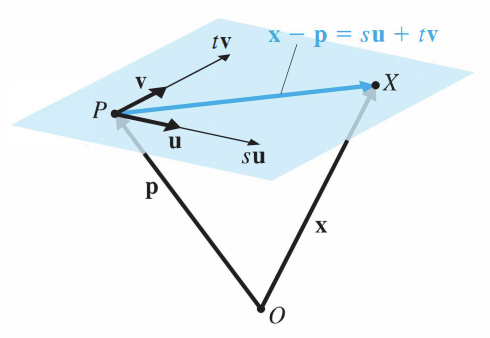
\includegraphics[scale=0.7]{VecPlane.png}
\caption{Defining a Plane with Vectors}
\label{vecplane}
\end{center}
\end{figure}
If we define the vectors as in Figure \ref{vecplane}, we can see that the distance from any general point $\vv{x}$ and $\vv{p}$ is just $\vv{x-p}$. Now notice how we can choose scalars $t$ and $s$ so that $s\vv{u} + t\vv{v} = \vv{x-p}$. Combining every possible combination of this defines the flat surface that is a plane. It follows that:
\begin{gather*}
    \vv{x} = \vv{p} + s\vv{u} + t\vv{v}
\end{gather*}
Looking at the figure, it makes sense why a single plane can't be defined with parallel direction vectors, since more than one plane could fit those conditions. Also note that plane is a 2 dimensional object, and requires two parameters to fully define it. For example, the parametric equation for $y$:
\begin{gather*}
    y = \vv{x}_y = \vv{p}_y + s\vv{u}_y + t\vv{v}_y
\end{gather*}
Since there are infinitely many lines in a plane, a line cannot be defined this way either. However, with two nonparallel normal vectors and a point, a line can defined as the set of points through $P$ perpendicular to $\vv{n}_1 $ and $\vv{n}_2$. Imagine a line being the $z$-axis, defined by two normal vectors off the $x$ and $y$ axis, with the point being the origin. Each normal vector can define it's own plane, so:
\begin{gather*}
    a_1x + b_1y + c_1z = d_1\\
    a_2x + b_2y + c_2z = d_2
\end{gather*}
The set of all $x,y,z$ that satisfy these two equations forms a line. Geometrically, this shows that the intersection of two planes forms a line.

Notice that a single equation of this type defines a different object as you increase dimensions. In $\mathbb{R}_2$, it defined a line. In $\mathbb{R}_3$, a plane, and in $R_n$, an $n-1$ dimension object called a \textit{hyperplane}. The relation between the dimension of an object $D_o$, the number of general equations required $E_o$, and the dimension of the space($D_s$) it is in:
\begin{gather*}
    D_o + E_o = D_s
\end{gather*}
This explains why the hyperplane defined by one equation is always one dimension lower than the space. It also explains why a line needs only one equation in $\mathbb{R}_2$ but two in $\mathbb{R}_3$.
\section{Systems of Linear Equations}
\end{document}
